% Created 2022-02-27 Sun 23:46
% Intended LaTeX compiler: pdflatex
\documentclass[12pt]{article}
\usepackage[utf8]{inputenc}
\usepackage[T1]{fontenc}
\usepackage{graphicx}
\usepackage{longtable}
\usepackage{wrapfig}
\usepackage{rotating}
\usepackage[normalem]{ulem}
\usepackage{amsmath}
\usepackage{amssymb}
\usepackage{capt-of}
\usepackage{hyperref}
\usepackage[margin=1in]{geometry}
\usepackage[backend=bibtex]{biblatex}
\addbibresource{./lab5.bib}
\author{Eric Nguyen \qquad Group 4}
\date{\today}
\title{Lab 5 - Superconductivity}
\hypersetup{
 pdfauthor={Eric Nguyen \qquad Group 4},
 pdftitle={Lab 5 - Superconductivity},
 pdfkeywords={},
 pdfsubject={},
 pdfcreator={Emacs 27.2 (Org mode 9.6)}, 
 pdflang={English}}
\begin{document}

\maketitle
\begin{abstract}
The goal of this experiment is to observe the resistance of a superconductor at low temperatures, expecting the resistance to approach zero past some transition temperature \(T_c\).
To enable measurement of the sample's resistivity at low temperatures, I make use of a cryostsat.
I found that the superconductor indeed reached a resistance of zero once cooled down enough past a certain \(T_c\).
\end{abstract}

\section*{Introduction}
\label{sec:orgd8fe36a}

One of the topics in recent physics literature that motivates the study of superconductors is that of topology and spin-orbit coupling.
This led to the discovery of topological insulators which support the idea `spinless' superconductivity. \cite{Sato_2017}

\section*{Experimental Method}
\label{sec:org923a4e0}

The experiment involves measuring the resistance across the BSCCO superconductor sample while its temperature cools down below the transition temperature \(T_c\) and then measure its resistance again while its temperature heats back up past the transition temperature \(T_c\).

\subsection*{Equipment}
\label{sec:org9b9e895}

Temperature variable cryostat, The BSCCO sample, Sample temperature indicator, Sample state temperature control, Bi-polar current source, Sample voltage amplifier, Sample stage heater power source

\begin{figure}[htbp]
\centering
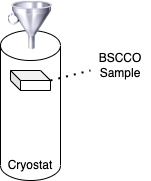
\includegraphics[width=120px]{./lab5.png}
\caption{Apparatus diagram of cryostat and BSCCO sample}
\end{figure}

\subsection*{Procedure}
\label{sec:orgf6f23ad}

First, I configured the voltage amplifier with the following settings: \textbf{Input Gain = 100}, \textbf{Second Stage Gain = 10}, \textbf{Time Constant = .1 Seconds}, and set input switches to \textbf{10M\(\Omega\)}.
Then, I measured the voltage across at sample bias currents of \(\pm 1 \text{ mA}\), \(\pm 10 \text{ mA}\), and \(\pm 100 \text{ mA}\) at room temperature.
Afterwards, I set the sample bias current to 100 mA and intermittently poured liquid nitrogen into cryostat through the funnel on top until the sample temperature reaches 85K, recording the voltage every 10 minutes or so.
Once the sample reached 85K, I started heating up the sample in small increments and once again measured its resistance.

\section*{Theoretical Background}
\label{sec:org02f850d}

To determine the voltage we need to obtain the desired sample temperature, we use the equation

\[V = 1146.4 - 0.4576T - 0.3476 T \ln{T}. \tag{1}\]

Then to determine the resistance across the sample, we measure voltage for both positive polarity \(V_+\) and negative polarity \(V_-\) and use the equation

\[\frac{1}{2} (V_+ - V_-) / GI_{\text{Bias}} \tag{2}\]

where \(G = 100\) is the input gain and \(I_{\text{Bias}}\) is the sample bias current.

\section*{Results and Analysis}
\label{sec:org61db0f2}

\begin{figure}[htbp]
\centering
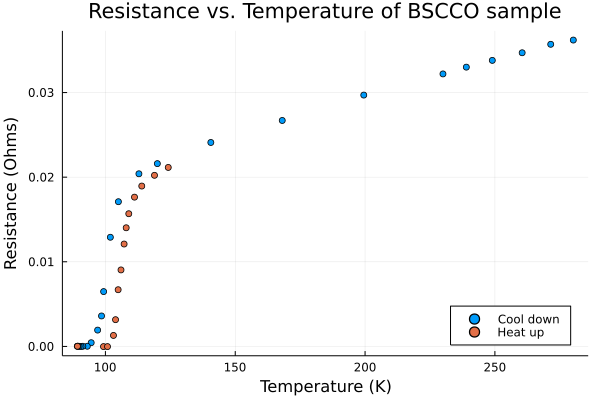
\includegraphics[width=.9\linewidth]{./resistancetemperature.png}
\caption{Resistance vs. temperature curve for superconductor BSCCO sample in both cooling down and heating up processes}
\end{figure}

\begin{table}[htbp]
\caption{Temperature and resistance data during cooling of BSCCO sample}
\centering
\begin{tabular}{rrrr}
Sample Temperature (K) & Voltage (V) Polarity + & Voltage (V) Polarity - & Resistance (Ohms)\\
\hline
280.2 & 1.800 & -1.820 & 0.0362\\
271.5 & 1.786 & -1.785 & 0.0357\\
260.5 & 1.723 & -1.748 & 0.0347\\
249.0 & 1.680 & -1.699 & 0.0338\\
239.0 & 1.638 & -1.657 & 0.0330\\
230.0 & 1.606 & -1.618 & 0.0322\\
199.5 & 1.486 & -1.481 & 0.0297\\
168.1 & 1.346 & -1.328 & 0.0267\\
140.6 & 1.220 & -1.186 & 0.0241\\
120.0 & 1.100 & -1.056 & 0.0216\\
112.9 & 1.042 & -0.993 & 0.0204\\
105.0 & 0.881 & -0.826 & 0.0171\\
101.9 & 0.679 & -0.613 & 0.0129\\
99.31 & 0.347 & -0.301 & 0.00648\\
98.50 & 0.170 & -0.190 & 0.00360\\
97.00 & 0.092 & -0.101 & 0.00193\\
94.52 & 0.014 & -0.030 & 0.00044\\
93.02 & -0.009 & -0.011 & 0.00002\\
91.31 & -0.011 & -0.013 & 0.00002\\
90.61 & -0.012 & -0.011 & -0.00001\\
89.90 & -0.008 & -0.009 & 0.00001\\
89.46 & -0.007 & -0.010 & 0.00003\\
89.16 & -0.012 & -0.014 & 0.00002\\
\end{tabular}
\end{table}

\begin{table}[htbp]
\caption{Temperature and resistance data during heating of BSCCO sample}
\centering
\begin{tabular}{rrrr}
Sample Temperature (K) & Voltage (V) Polarity + & Voltage (V) Polarity - & Resistance (Ohms)\\
\hline
89.24 & -0.010 & -0.012 & 0.00002\\
99.26 & -0.010 & -0.008 & -0.00002\\
100.8 & -0.011 & -0.009 & -0.00002\\
103.1 & 0.054 & -0.076 & 0.0013\\
103.9 & 0.146 & -0.170 & 0.00316\\
104.9 & 0.323 & -0.347 & 0.00670\\
106.0 & 0.440 & -0.464 & 0.00904\\
107.2 & 0.593 & -0.617 & 0.01210\\
108.0 & 0.689 & -0.713 & 0.01402\\
109.0 & 0.772 & -0.796 & 0.01568\\
111.2 & 0.868 & -0.896 & 0.01764\\
114.0 & 0.933 & -0.962 & 0.01895\\
118.9 & 0.996 & -1.026 & 0.02022\\
124.2 & 1.043 & -1.072 & 0.02115\\
\end{tabular}
\end{table}

While in both the cooling down and heating up processes the resistance versus temperature curve share a similar shape, the curves do not overlap with one another.
The most likely reason for this is that the resistance starts increasing at a higher temperature when the sample is heating up while the resistance reaches zero at a lower temperature for when the sample is cooling down.
Indeed, the difference appears to be a shift in temperatures starting from the initial transition temperature \(T_{c_0}\) to the onset transition temperature \(T_{c_{\text{onset}}}\).

\section*{Conclusion}
\label{sec:org65df817}

I found that the BSCCO sample indeed is a superconductor.
That is, the sample's resistance reached zero after it's temperature dropped below a certain transition temperature.


\printbibliography
\end{document}
